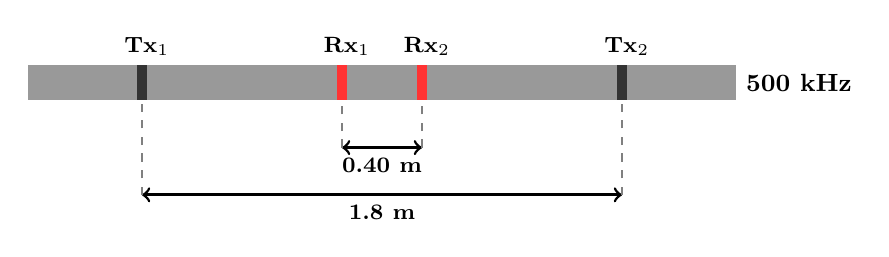
\begin{tikzpicture}

%% Tool
\fill[gray!80!white] (-1.5*3,0) -- (1.5*3,0.) --  node[right] {\small \bf \textcolor{black}{500 kHz}}  (1.5*3, 0.15*3) -- (-1.5*3,0.15*3) -- cycle;

%% Transmitters
\fill[black!80!white] (-0.6096*5-0.02*3,0) -- (-0.6096*5+0.02*3,0.) -- (-0.6096*5+0.02*3, 0.15*3) node[above] {\footnotesize \bf \textcolor{black}{Tx$_1$}}  -- (-0.6096*5-0.02*3,0.15*3) -- cycle;
%
\fill[black!80!white] (0.6096*5-0.02*3,0) -- (0.6096*5+0.02*3,0.)  -- (0.6096*5+0.02*3, 0.15*3) node[above] {\footnotesize \bf \textcolor{black}{Tx$_2$}} -- (0.6096*5-0.02*3,0.15*3) -- cycle;

%% Receivers
\fill[red!80!white] (-0.1016*5-0.02*3,0) -- (-0.1016*5+0.02*3,0.)  -- (-0.1016*5+0.02*3, 0.15*3) node[above] {\footnotesize \bf \textcolor{black}{Rx$_1$}} -- (-0.1016*5-0.02*3,0.15*3) -- cycle;
\fill[red!80!white] ( 0.1016*5-0.02*3,0) -- ( 0.1016*5+0.02*3,0.) -- ( 0.1016*5+0.02*3, 0.15*3)  node[above] {\footnotesize \bf \textcolor{black}{Rx$_2$}} -- ( 0.1016*5-0.02*3,0.15*3) -- cycle;

%% distances
\draw[black, line width=1pt,<->] (-0.1016*5, -0.6)      -- (0.1016*5, -0.6) node[pos=0.5, below] {\footnotesize \bf \textcolor{black}{0.40 m}}  ;
\draw[gray, dashed] (-0.1016*5, -0.6)      -- (-0.1016*5, 0)  ;
\draw[gray, dashed] ( 0.1016*5, -0.6)      -- ( 0.1016*5, 0)  ;

\draw[black, line width=1pt,<->] (-0.6096*5, -1.2)      -- (0.6096*5, -1.2) node[pos=0.5, below] {\footnotesize \bf \textcolor{black}{1.8 m}}  ;
\draw[gray, dashed] (-0.6096*5,-1.2)      -- (-0.6096*5, 0)  ;
\draw[gray, dashed] ( 0.6096*5,-1.2)      -- ( 0.6096*5, 0)  ;


\end{tikzpicture}